\hypertarget{ux5faaux73afux795eux7ecfux7f51ux7edc}{%
\chapter{循环神经网络}\label{ux5faaux73afux795eux7ecfux7f51ux7edc}}

\hypertarget{ux81eaux56deux5f52ux6a21ux578b}{%
\section{自回归模型}\label{ux81eaux56deux5f52ux6a21ux578b}}

\hypertarget{ux4e00ux6838ux5fc3ux601dux60f3}{%
\subsection{一、核心思想}\label{ux4e00ux6838ux5fc3ux601dux60f3}}

一个序列中当前时刻的值，可以由其过去若干个时刻的值的线性组合加上一个随机扰动（误差）来解释和预测。如基于这个上下文来预测最可能出现的``下一个''词。

一个~p阶~的自回归模型，记为~AR(p)，其公式定义为：

\[
X_t = c + \phi_1 X_{t-1} + \phi_2 X_{t-2} + \cdots + \phi_p X_{t-p} + \epsilon_t
\]

公式解读：

\begin{itemize}
\tightlist
\item
  \(X_t\)：当前时刻 \(t\) 的变量值（我们想要预测的值）。
\item
  \(c\)：常数项（截距）。
\item
  \(\phi_1, \phi_2, \ldots, \phi_p\)：自回归系数。这些是模型需要学习的参数，代表了过去每个时刻的值对当前值的影响程度和方向。
\item
  \(X_{t-1}, X_{t-2}, \ldots, X_{t-p}\)：过去 \(p\) 个时刻的历史值。
\item
  \(\epsilon_t\)：时刻 \(t\) 的随机误差项（白噪声）。它代表了模型无法用历史数据解释的随机波动，通常假设其均值为 0，方差恒定。
\end{itemize}

阶数 p决定了模型回看多远的过去。p 的选择至关重要，太小可能欠拟合，太大可能过拟合。

平稳性要求：序列的均值、方差和协方差不随时间推移而发生显著变化。如果不平稳，通常需要通过差分等方法将其转换为平稳序列（这就引出了ARIMA模型中的``I''）。

\hypertarget{ux4e8cux5e94ux7528}{%
\subsection{二、应用}\label{ux4e8cux5e94ux7528}}

\begin{enumerate}
\def\labelenumi{\arabic{enumi}.}
\tightlist
\item
  LLM：将生成问题看作一个序列生成问题（词序列、token序列）。模型定义了一个条件概率分布：\(P(x_t | x_{<t})\)。即，给定所有已经生成的词 \(x_1, x_2, ..., x_{t-1}\)，计算下一个词 \(x_t\) 的概率分布。从该分布中采样（或取最可能）得到下一个词 \(x_t\)。将新生成的词 \(x_t\) 加入上下文，重复步骤，直到生成序列结束符或达到最大长度。
\end{enumerate}

实现技术：~通过掩码机制（Causal Masking）~实现。在Transformer中，确保在计算第t个位置的注意力时，只能``看到''第1到第t-1个位置的信息，无法看到``未来''的信息，从而严格保证了自回归的特性。

\begin{enumerate}
\def\labelenumi{\arabic{enumi}.}
\setcounter{enumi}{1}
\tightlist
\item
  计算机视觉：也可以用``给定之前所有生成的概率，预测下一个像素的概率分布''的方法生成非常清晰、高质量的图像，但缺点是非常慢，因为必须逐个像素顺序生成，无法并行。
\end{enumerate}

\hypertarget{ux53c2ux8003ux6587ux732e-15}{%
\subsection{参考文献}\label{ux53c2ux8003ux6587ux732e-15}}

\begin{itemize}
\tightlist
\item
  Aston Zhang, Zachary C. Lipton, Mu Li, Alexander J. Smola. (2023). \href{https://zh.d2l.ai/}{《动手学深度学习》}. Cambridge University Press.
\end{itemize}

\clearpage

\hypertarget{ux5faaux73afux795eux7ecfux7f51ux7edcrnn}{%
\section{循环神经网络（RNN）}\label{ux5faaux73afux795eux7ecfux7f51ux7edcrnn}}

\hypertarget{ux4e00ux6838ux5fc3ux601dux60f3-1}{%
\subsection{一、核心思想}\label{ux4e00ux6838ux5fc3ux601dux60f3-1}}

RNN的核心思想是为网络引入``记忆''或``状态''的概念，使其能够保留之前输入的信息，并用于影响当前输出的计算。

前馈神经网络（如CNN、MLP）假设所有输入（和输出）之间是相互独立的。处理一个输入样本时，不会考虑它之前或之后的样本，没有``上下文''的概念。每次前向计算时，输入的样本的数据量是恒定的。对于基于此设计的 \(n\) 元语法模型（\(n\) 给定），要预测下一个词 \(x_t\)，它只会回头看紧挨着的前 \(n-1\) 个词 \(x_{t-1},\ldots,x_{t-n+1}\)，但如果 \(n\) 变得很大，模型需要记录所有可能的 \(n\) 个词组合的概率。假设词表有10万个词，一个 \(n=4\) 的模型就需要存储 \(100{,}000^4\) 个概率值，这是一个天文数字，在计算和存储上都是不可能的。

为了解决 \(n\) 增大带来的参数爆炸问题，我们引入一个隐变量模型。这个模型不再直接依赖于所有过去的历史词，而是依赖于一个总结了过去所有历史信息的中间变量，称为隐状态（hidden state）。新的模型化为：

\[
P(x_t \mid x_{t-1},\ldots,x_1) \approx P(x_t \mid h_{t-1})
\]

这个隐状态 \(h_{t-1}\) 是一个向量，它封装了从序列开始到 \(t-1\) 时刻的所有有用信息。它的维度是固定的（比如256维），不会因为序列变长而改变大小。这就巧妙地避免了参数随历史长度指数增长。基于此设计的循环神经网络（RNN）专门设计用于处理序列数据，即输入（或输出）是一个接一个的、相互关联的数据点。例如时间序列数据（股票价格、天气数据、传感器读数）、自然语言（句子、段落，本质上是词的序列）、音频/视频（按时间顺序排列的帧或采样点）。

\hypertarget{ux4e8cux6570ux5b66ux8868ux8fbe}{%
\subsection{二、数学表达}\label{ux4e8cux6570ux5b66ux8868ux8fbe}}

\begin{enumerate}
\def\labelenumi{\arabic{enumi}.}
\tightlist
\item
  新的隐藏层：
\end{enumerate}

\[
h_t=f(x_t,h_{t-1})=\phi(W_{xh}x_t+W_{hh}h_{t-1}+b_h)
\]

\(W_{xh}x_t\)：这是一个线性变换，将当前输入 \(x_t\)（一个代表词的数字向量）投影到隐藏空间。

\(W_{hh}h_{t-1}\)：这是另一个线性变换，将过去的隐状态（记忆）也投影到隐藏空间。权重矩阵 \(W_{hh}\) 是RNN最关键的部分，它决定了过去的记忆如何影响当前状态。

\(b_h\)：偏置项。

\(\phi\)：一个非线性激活函数（如 \(\tanh\) 或ReLU）。\(\tanh\) 函数可以将值压缩到 \((-1,1)\) 之间，有助于稳定网络的输出。

\begin{enumerate}
\def\labelenumi{\arabic{enumi}.}
\setcounter{enumi}{1}
\tightlist
\item
  生成输出：新的隐藏状态 \(h_t\) 通常可以直接用作输出，或者再通过一个输出层进行计算。当前时刻的最终输出为：
\end{enumerate}

\[
o_t=W_{ho}h_t+b_o
\]

\begin{enumerate}
\def\labelenumi{\arabic{enumi}.}
\setcounter{enumi}{2}
\tightlist
\item
  参数更新：通过时间反向传播（BPTT）
\end{enumerate}

（1）将网络按时间步展开成一个深度的前馈网络

想象RNN在处理一个长度为5的序列 \([x_1,x_2,x_3,x_4,x_5]\)。前向传播时，RNN逐步计算：

\[
h_1=f(x_1,h_0)\to h_2=f(x_2,h_1)\to h_3=f(x_3,h_2)\to h_4=f(x_4,h_3)\to h_5=f(x_5,h_4)
\]

BPTT的视角：它把这个过程看成是一个5层的特殊DNN：

第1层：输入是 \([x_1,h_0]\)，输出是 \(h_1\)

第2层：输入是 \([x_2,h_1]\)，输出是 \(h_2\)

\ldots{}

这个``深度网络''的特殊之处在于：所有``层''都共享同一组参数 \((W_{xh}, W_{hh}, b_h)\)。第 \(t\) 层的输入不仅包括原始输入 \(x_t\)，还包括前一层的输出 \(h_{t-1}\)。

（2）反向传播

我们以一个简单的 RNN 为例，其隐状态更新公式为：

\[
h_t = \tanh(W_{xh}x_t + W_{hh}h_{t-1} + b_h)
\]

最终输出和损失为：

\[
o_t = W_{hq}h_t + b_q
\]

\[
L = \sum_{t=1}^{T} L_t = \sum_{t=1}^{T} \mathrm{Loss}(o_t, y_t)
\]

A. 计算最终输出层参数的梯度（\(W_{hq}, b_q\)）

这部分最简单，因为 \(o_t\) 只依赖于 \(h_t\)，梯度不跨时间步传播，可以按时间步独立计算再求和。

\[
\frac{\partial L}{\partial W_{hq}}
= \sum_{t=1}^{T} \frac{\partial L_t}{\partial o_t}\frac{\partial o_t}{\partial W_{hq}}
= \sum_{t=1}^{T}(o_t - y_t) \cdot h_t^T
\]

\[
\frac{\partial L}{\partial b_q}
= \sum_{t=1}^{T} \frac{\partial L_t}{\partial o_t}\frac{\partial o_t}{\partial b_q}
= \sum_{t=1}^{T}(o_t - y_t)
\]

B. 计算循环层参数的梯度（\(W_{xh}, W_{hh}, b_h\)）

总损失 \(L\) 依赖于 \(h_t\)，而 \(h_t\) 又依赖于 \(h_{t-1}\) 和参数，这种依赖关系一直传递到序列开始。因此，梯度计算涉及跨时间步的链式法则。

我们定义一个关键变量：损失对 \(t\) 时刻隐状态的梯度 \(\delta_t\)。

\[
\delta_t = \frac{\partial L}{\partial h_t}
\]

\begin{enumerate}
\def\labelenumi{\arabic{enumi}.}
\tightlist
\item
  从最后一个时间步 \(T\) 开始初始化：
\end{enumerate}

\(\delta_T\) 由两部分构成：来自当前输出的损失和来自未来的损失。但在许多简单情况下，如果 \(h_T\) 只影响 \(o_T\)，则：

\[
\delta_T = \frac{\partial L_T}{\partial h_T}
= \frac{\partial L_T}{\partial o_T}\frac{\partial o_T}{\partial h_T}
= (o_T - y_T) W_{hq}^T
\]

\begin{enumerate}
\def\labelenumi{\arabic{enumi}.}
\setcounter{enumi}{1}
\tightlist
\item
  对于 \(t = T-1, T-2, \ldots, 1\)，梯度递归地反向传播：
\end{enumerate}

\[
\delta_t = \frac{\partial L_t}{\partial h_t} + \frac{\partial h_{t+1}}{\partial h_t}\delta_{t+1}
\]

其中，第一项来自当前输出，第二项来自未来时间步。

\hypertarget{ux4e09ux4f20ux7edfrnnux5b58ux5728ux7684ux95eeux9898grulstmux7684ux63d0ux51faux80ccux666f}{%
\subsection{三、传统RNN存在的问题（GRU、LSTM的提出背景）}\label{ux4e09ux4f20ux7edfrnnux5b58ux5728ux7684ux95eeux9898grulstmux7684ux63d0ux51faux80ccux666f}}

\begin{enumerate}
\def\labelenumi{\arabic{enumi}.}
\tightlist
\item
  梯度消失与梯度爆炸
\end{enumerate}

这是RNN最著名的问题。在反向传播时，梯度需要沿着时间步一路相乘回去。

如果 \(W_{hh}\)（隐藏状态权重矩阵）的特征值小于1，连续相乘会导致梯度变得极小，以至于较早时间步的参数无法得到有效更新，难以修正其在序列早期犯下的错误（网络``忘记''了远处的事情）。而如果想强行让模型记住早期信息，就需要早期参数产生一个在反向传播中不衰减的巨大梯度，这要么在数学上很难自然发生，要么会引发另一个问题（引发梯度爆炸，影响其他参数训练）导致训练失败。

反之，如果特征值大于1，梯度会指数级增长（梯度爆炸），导致训练不稳定，网络参数更新剧烈，无法收敛。

\begin{enumerate}
\def\labelenumi{\arabic{enumi}.}
\setcounter{enumi}{1}
\tightlist
\item
  长程依赖问题
\end{enumerate}

梯度消失的直接后果就是模型难以学习到序列中远距离的依赖关系。例如，在句子``The clouds which have been covering the sky all day are finally starting to \_\_\_''中，要预测最后一个词``clear''或``rain''，模型需要记住很久之前的主语``clouds''。

传统RNN的困境：由于梯度消失，网络很难将第一个时间步的信息（误差）一路传递到最后一个时间步。为了学会记住这个信息，网络必须给第一个时间步分配一个巨大的梯度，这在实际训练中很难实现。

所需的机制：需要一个``记忆单元''，能够像计算机硬盘一样，稳定地存储关键信息很长一段时间，而不受后续操作（梯度计算）的干扰。

\begin{enumerate}
\def\labelenumi{\arabic{enumi}.}
\setcounter{enumi}{2}
\tightlist
\item
  难以满足忽略无关信息需求
\end{enumerate}

例子：在分析网页情感时，HTML标签（如 \texttt{\textless{}div\textgreater{}}、\texttt{\textless{}br\textgreater{}}）与情感无关，是噪声。

传统RNN的困境：传统RNN会无差别地处理每一个输入，这些无关词元也会更新隐状态，污染后续有用的信息。

所需的机制：需要一个``遗忘''或``跳过''机制，能够主动选择哪些信息是重要的需要流入，哪些是不重要的需要被忽略。

\begin{enumerate}
\def\labelenumi{\arabic{enumi}.}
\setcounter{enumi}{3}
\tightlist
\item
  难以满足重置内部状态需求
\end{enumerate}

例子：序列的不同部分之间存在明显边界或主题转换，比如书的新章节开始，或市场行情从熊市转为牛市。

传统RNN的困境：传统RNN的隐状态会不断地累积历史信息。当场景突然切换时，旧章节或旧行情的信息会持续影响新章节或新行情的学习，造成干扰。

所需的机制：需要一个``重置''机制，能够在检测到逻辑中断时，有选择地清除过去的、不再相关的记忆，从而更好地初始化新场景的学习。

\hypertarget{ux53c2ux8003ux6587ux732e-16}{%
\subsection{参考文献}\label{ux53c2ux8003ux6587ux732e-16}}

\begin{itemize}
\tightlist
\item
  Aston Zhang, Zachary C. Lipton, Mu Li, Alexander J. Smola. (2023). \href{https://zh.d2l.ai/}{《动手学深度学习》}. Cambridge University Press.
\end{itemize}

\clearpage

\hypertarget{ux7f16ux7801ux5668-ux89e3ux7801ux5668ux67b6ux6784}{%
\section{编码器-解码器架构}\label{ux7f16ux7801ux5668-ux89e3ux7801ux5668ux67b6ux6784}}

编码器-解码器（Encoder-Decoder）架构的目标是将一个输入序列（例如一句英文句子）(x₁, x₂, \ldots, x\_T)~转换成一个输出序列（例如一句中文句子）(y₁, y₂, \ldots, y\_T')。两个序列的长度可以不同。

编码器：读取并``理解''整个输入序列，将其压缩成一个固定维度的上下文向量（Context Vector）~c，这个向量旨在包含输入序列的完整语义信息。

解码器：以该上下文向量~c~作为初始``记忆''和``指令''，开始逐步生成输出序列。

\hypertarget{ux4e00ux7f16ux7801ux5668encoder}{%
\subsection{一、编码器（Encoder）}\label{ux4e00ux7f16ux7801ux5668encoder}}

编码器是一个RNN（可以是普通RNN、LSTM或GRU）。它逐个处理输入序列中的每个词元。

对于每一个时间步~t~(从 1 到~T)，编码器执行以下计算：
h\_t\^{}\{enc\} = f\_\{enc\}(x\_t, h\_\{t-1\}\^{}\{enc\})

h\_t\^{}\{enc\}： 编码器在时间步~t~的隐状态。

f\_\{enc\}： 编码器RNN的函数（例如，LSTM单元的计算过程）。它包含可学习的参数~W\_\{xh\}\textsuperscript{\{enc\},~W\_\{hh\}}\{enc\},~b\_h\^{}\{enc\}~等以及激活函数。

x\_t： 时间步~t~的输入词嵌入向量。

h\_\{t-1\}\^{}\{enc\}： 上一个时间步的隐状态。初始隐状态~h\_0\^{}\{enc\}~通常初始化为全零向量。

上下文向量的生成：
在处理完整个输入序列后，编码器最后一个时间步的隐状态~h\_T\^{}\{enc\}~被用作上下文向量~c。
c = h\_T\^{}\{enc\}

这个向量~c~承载了编码器从整个输入序列中读取并整合的所有信息。它将被用作解码器的初始状态。

更高级的架构中，c~可以是一个池化后的结果，或者是注意力机制的加权组合，但最经典的形式就是~h\_T\^{}\{enc)。

\hypertarget{ux4e8cux89e3ux7801ux5668decoder}{%
\subsection{二、解码器（Decoder）}\label{ux4e8cux89e3ux7801ux5668decoder}}

解码器是另一个RNN，其目标是生成输出序列。它的初始状态由编码器提供的上下文向量初始化。

数学表达：解码器在每一个时间步~t'~(从 1 到~T') 的计算分为两部分：

\begin{enumerate}
\def\labelenumi{\alph{enumi})}
\tightlist
\item
  计算当前隐状态：
  s\_\{t'\} = f\_\{dec\}(y\_\{t'-1\}, s\_\{t'-1\})
\end{enumerate}

s\_\{t'\}： 解码器在时间步~t'~的隐状态。

f\_\{dec\}： 解码器RNN的函数，参数~W\_\{xh\}\textsuperscript{\{dec\},~W\_\{hh\}}\{dec\},~b\_h\^{}\{dec\}~等。

s\_\{t'-1\}： 解码器上一个时间步的隐状态。关键点：初始状态~s\_0~被设置为上下文向量~c。
s\_0 = c

y\_\{t'-1\}：~解码器在上一个时间步~生成~的输出。在训练和推理时，这个输入的策略不同（详见后面的`` teacher forcing''）。

\begin{enumerate}
\def\labelenumi{\alph{enumi})}
\setcounter{enumi}{1}
\tightlist
\item
  计算当前输出：
  解码器的隐状态~s\_\{t'\}~被送入一个输出层（通常是全连接层 + Softmax），以预测当前时间步的输出词元概率分布。
  o\_\{t'\} = g(s\_\{t'\}) = \text{softmax}(W\_\{out\} s\_\{t'\} + b\_\{out\})
  P(y\_\{t'\} \textbar{} y\_\{\textless t'\}, c) = o\_\{t'\}
\end{enumerate}

o\_\{t'\}： 一个概率分布向量，其维度与输出词表大小相同。每个值代表了对应词元是当前时间步~t'~输出的概率。一般而言，每个词由

W\_\{out\},~b\_\{out\}： 输出层的权重和偏置参数。

解码器生成序列的过程是一个自回归（Autoregressive）过程：

初始状态~s\_0 = c，初始输入通常是一个特殊的~token。

计算~s\_1~和~o\_1，从~o\_1~中采样或取argmax得到第一个词~y₁。

将~y₁~作为下一个时间步的输入，计算~s\_2~和~o\_2，得到~y₂。

重复此过程，直到生成一个特殊的~token，表示序列生成结束。

\hypertarget{ux4e09ux603bux7ed3ux4e0eux5b8cux6574ux7684ux6570ux5b66ux6d41ux7a0b}{%
\subsection{三、总结与完整的数学流程}\label{ux4e09ux603bux7ed3ux4e0eux5b8cux6574ux7684ux6570ux5b66ux6d41ux7a0b}}

将一个输入序列~X = (x₁, x₂, \ldots, x\_T)~翻译为输出序列~Y = (y₁, y₂, \ldots, y\_\{T'\})：

\begin{enumerate}
\def\labelenumi{\arabic{enumi}.}
\item
  编码器阶段：
  h\_t\^{}\{enc\} = f\_\{enc\}(x\_t, h\_\{t-1\}\^{}\{enc\}), \quad \text{for } t = 1, \ldots, T
  c = h\_T\^{}\{enc\}
\item
  解码器阶段：
  s\_0 = c
  s\_\{t'\} = f\_\{dec\}(y\_\{t'-1\}, s\_\{t'-1\}), \quad \text{for } t' = 1, \ldots, T'
  P(y\_\{t'\} \textbar{} y\_\{\textless t'\}, c) = g(s\_\{t'\}) = \text{softmax}(W\_\{out\} s\_\{t'\} + b\_\{out\})
\item
  训练目标和损失：
  最大化输出序列的条件对数似然：
  要log P(Y\textbar X) 最大，也就是sum(log P(y\_\{t'\} \textbar{} y\_\{\textless t'\})最大；而-log P(y\_\{t'\} \textbar{} y\_\{\textless t'\})就是交叉熵损失，让模型趋向于真实one-hot分布
\item
  一个重要技巧：Teacher Forcing
\end{enumerate}

在训练时，解码器每一步的输入~y\_\{t'-1\}~有一个重要选择：

不使用Teacher Forcing： 使用解码器自己上一步预测的结果作为输入。错误会累积，训练可能不稳定。

使用Teacher Forcing： 无论解码器上一步预测的是什么，都强制使用真实标签（Ground Truth）~中的上一个词~y\_\{t'-1\}\^{}\{true\}~作为输入。

s\_\{t'\} = f\_\{dec\}(y\_\{t'-1\}\^{}\{true\}, s\_\{t'-1\})

这大大加速了训练的收敛，因为它在每一步都为解码器提供了正确的上下文。然而，这可能导致训练和推理时的不匹配（Exposure Bias），因为推理时没有真实标签可用。通常采用一种课程学习策略，在训练后期逐渐减少Teacher Forcing的使用。

推理时，则没有真实标签可用，只能使用解码器自己上一步的预测结果作为当前步的输入。

\hypertarget{ux53c2ux8003ux6587ux732e-17}{%
\subsection{参考文献}\label{ux53c2ux8003ux6587ux732e-17}}

\begin{itemize}
\tightlist
\item
  Aston Zhang, Zachary C. Lipton, Mu Li, Alexander J. Smola. (2023). \href{https://zh.d2l.ai/}{《动手学深度学习》}. Cambridge University Press.
\end{itemize}

\clearpage

\hypertarget{ux95e8ux63a7ux8bb0ux5fc6ux5355ux5143gru}{%
\section{门控记忆单元（GRU）}\label{ux95e8ux63a7ux8bb0ux5fc6ux5355ux5143gru}}

\hypertarget{ux4e00ux57faux672cux539fux7406}{%
\subsection{一、基本原理}\label{ux4e00ux57faux672cux539fux7406}}

\begin{enumerate}
\def\labelenumi{\arabic{enumi}.}
\tightlist
\item
  重置门~R\_t：控制``可能还想记住''的过去状态的数量。它决定了有多少过去的信息需要被``忘记''（如网页中html码等无用信息，我们不希望其参与候选状态计算），以便与新输入结合形成新的候选状态。
\end{enumerate}

重置门有助于捕获序列中的短期依赖关系。它通过控制有多少过去信息参与新候选状态的计算，来影响当前时刻的即时反应。这对于理解紧邻词元之间的关系（短期模式）非常有效。

\begin{enumerate}
\def\labelenumi{\arabic{enumi}.}
\setcounter{enumi}{1}
\tightlist
\item
  更新门~Z\_t：控制新状态中旧状态和候选状态的比例。它决定了有多少过去的信息会被直接保留到新的状态中（如一些必须原样保留的信息）。
\end{enumerate}

更新门~有助于捕获序列中的长期依赖关系。它通过控制信息传递的路径，让网络能够直接复制过去的状态。如果模型学到让更新门在很长一段时间内都保持接近1，那么很久以前的信息就可以几乎无损地传递到未来，从而完美地解决了梯度消失问题，擅长捕捉长期模式。

接下来，GRU 不是直接计算新的隐状态，而是先计算一个候选隐状态（Candidate Hidden State）\(\tilde{H}_t\)。这个候选状态表示在当前输入和经过筛选的过去信息共同作用下可能形成的新状态。

重置门 \(R_t\) 在这里起到关键作用：它通过与前一状态 \(H_{t-1}\) 进行按元素乘法（Hadamard 积）来``重置''或``过滤''过去的信息。

\begin{itemize}
\tightlist
\item
  如果重置门 \(R_t\) 的某个元素接近 1，则表示允许对应的过去信息通过，公式退化为类似传统 RNN 的更新方式 \(\tanh(X_t W_{xh} + H_{t-1}W_{hh} + b_h)\)。
\item
  如果重置门 \(R_t\) 的某个元素接近 0，则会``屏蔽''或``忘记''对应的过去信息。此时，候选状态仅由当前输入 \(X_t\) 决定（类似于一个简单的 MLP），这有助于忽略无关信息。
\end{itemize}

公式为：

\[
\tilde{H}_t = \tanh(X_t W_{xh} + (R_t \odot H_{t-1})W_{hh} + b_h)
\]

其中，\(\odot\) 表示 Hadamard 积（按元素相乘），\(\tanh\) 激活函数确保候选状态的值在 \((-1, 1)\) 之间。

最后，新的隐状态 \(H_t\) 是旧状态 \(H_{t-1}\) 和候选状态 \(\tilde{H}_t\) 之间的凸组合，这个组合的比例由更新门 \(Z_t\) 控制。

\begin{itemize}
\tightlist
\item
  如果更新门 \(Z_t\) 的某个元素接近 1，则新状态会大量保留旧状态的信息，几乎忽略掉候选状态（即当前输入的影响很小）。这使得网络能够跳过不重要的时间步，从而有效地将很久以前的信息传递下去，解决长期依赖问题。
\item
  如果更新门 \(Z_t\) 的某个元素接近 0，则新状态会更倾向于采用候选状态，即更多地关注当前输入。
\end{itemize}

这种机制使得 GRU 可以灵活地选择是``记住''长期信息还是``关注''短期输入。

公式为：

\[
H_t = Z_t \odot H_{t-1} + (1 - Z_t) \odot \tilde{H}_t
\]

形象理解：

GRU~像一个高效的现代工作站：

重置门：在思考新方案(\textasciitilde h\_t)前，先清空一下白板上不相关的内容。

更新门：决定最终的白板(h\_t)上，要擦掉多少旧内容，又要把新方案写上去多少。

两个思考的问题：

\begin{enumerate}
\def\labelenumi{\arabic{enumi}.}
\tightlist
\item
  为什么这里要单独用门，而不是直接调控权重？
\end{enumerate}

因为门有一个重要的特性：``按元素乘''

在传统矩阵乘法中，调一个权重必然涉及到与之相乘的所有元素，因而想通过这一方式保留或抹去特定位置的信息是很难的。门中的元素则和神经元一一对应。

\begin{enumerate}
\def\labelenumi{\arabic{enumi}.}
\setcounter{enumi}{1}
\tightlist
\item
  为什么两个门不能相互替代？
\end{enumerate}

如果只有重置门，没有更新门，候选隐状态计算函数很难直接拟合恒等变换y=x，无法保证信息原样传递；如果只有更新门，没有重置门，个别元素上的无关信息就会影响候选状态（因为前面讲过的原因，不能把对应权重直接设为0）。

\hypertarget{ux4e8cux91cdux7f6eux95e8ux4e0eux66f4ux65b0ux95e8ux7684ux8ba1ux7b97}{%
\subsection{二、重置门与更新门的计算}\label{ux4e8cux91cdux7f6eux95e8ux4e0eux66f4ux65b0ux95e8ux7684ux8ba1ux7b97}}

对于给定的时间步 \(t\)：

\[
R_t = \sigma(X_t W_{xr} + H_{t-1}W_{hr} + b_r)
\]

\[
Z_t = \sigma(X_t W_{xz} + H_{t-1}W_{hz} + b_z)
\]

其中：

\begin{itemize}
\tightlist
\item
  \(\sigma\) 是 sigmoid 激活函数。
\item
  \(W_{xr}, W_{xz}\) 是与输入 \(X_t\) 相乘的权重矩阵。
\item
  \(W_{hr}, W_{hz}\) 是与前一隐状态 \(H_{t-1}\) 相乘的权重矩阵。
\item
  \(b_r, b_z\) 是偏置参数。
\end{itemize}

那么，重置门和更新门为什么要由当前时间步的输入 X\_t 和前一个时间步的隐状态 H\_\{t-1\} 通过一个全连接层，再经过 sigmoid 激活函数计算得到？

\begin{enumerate}
\def\labelenumi{\arabic{enumi}.}
\tightlist
\item
  目的：门控需要成为``情境感知''的决策器
  这两个门在每个时刻都要做两个关键决策：
\end{enumerate}

重置门：为了处理好眼前这个新输入，我该忘掉多少刚才还记得的背景信息？

更新门：我是应该 mostly 记住旧的，还是应该~mostly 相信新的？

这些决策绝不能是死板的规则，必须根据当前具体遇到什么词、处在什么上下文环境中来灵活决定。

举个例子（情感分析）：
句子是：``This movie is not good at all, it is actually terribly boring.''

当模型读到~``not''~这个词时：

重置门应该意识到：下一个词~``good''~的意思要反转了！必须弱化/重置掉之前~``is''~带来的正面预感，准备好接收一个被否定后的信息。

更新门应该意识到：``not''~是个超级重要的信号！必须牢牢记住这个状态，把它强有力地传递下去，影响后面所有词的判断。

如果门控是固定的或者只由当前词决定，它就无法根据整个句子的上下文（由过去的隐藏状态编码）来做出如此精细和关键的决策。

所以，门控的决策必须基于两大信息源：

当前观测 (X\_t)：我现在看到了什么词？

历史上下文 (H\_\{t-1\})：我之前读到过什么，正处于什么样的理解背景下？

只有把这两者结合起来，门控才能做出最明智的、懂场景的（Context-Aware）~决策。

\begin{enumerate}
\def\labelenumi{\arabic{enumi}.}
\setcounter{enumi}{1}
\tightlist
\item
  结构：让模型自己学会权衡
  将当前输入和过去状态分别乘以权重再加起来，这个结构（称为``仿射变换''）是在让模型自己通过训练数据学习：在面对什么样的情况下，应该更相信当前输入；在什么样的情况下，应该更依赖历史记忆。
\end{enumerate}

对于能颠覆语义的词（如~``not'',~``but''），模型会学会让当前输入的权重很大，从而让当前词主导门的开关。

对于不重要的词（如~``the'',~``a''），模型会学会让历史状态的权重占主导，从而命令门控：``忽略它，保持原状！''

这种设计给了模型极大的灵活性。

\begin{enumerate}
\def\labelenumi{\arabic{enumi}.}
\setcounter{enumi}{2}
\tightlist
\item
  激活函数：Sigmoid------完美的``比例调节器''
  Sigmoid函数是一个神奇的``压缩器''，它能把任何大小的数字都变成一个介于0和1之间的值。
\end{enumerate}

完美的解释性：输出是0到1之间，可以天然地理解为~``开度的百分比''。比如：0是``全关''，1是``全开''，0.7是``开七成''。

可训练性：这个函数是光滑的，这对于使用反向传播算法来训练模型至关重要，误差可以顺利地通过它传回去调整权重。

清晰的决策：虽然它在极端情况下会饱和（导致梯度消失），但在门控这里这反而是个优点。它允许门的输出无限接近0或1，从而实现非常坚决的``开''或``关''的决策，形成稳定的记忆流。

\hypertarget{ux4e09ux603bux7ed3}{%
\subsection{三、总结}\label{ux4e09ux603bux7ed3}}

通过重置门和更新门的协同工作，GRU能够动态地、有选择地管理记忆，从而在各种序列建模任务中取得优异的效果。

\hypertarget{ux53c2ux8003ux6587ux732e-18}{%
\subsection{参考文献}\label{ux53c2ux8003ux6587ux732e-18}}

\begin{itemize}
\tightlist
\item
  Aston Zhang, Zachary C. Lipton, Mu Li, Alexander J. Smola. (2023). \href{https://zh.d2l.ai/}{《动手学深度学习》}. Cambridge University Press.
\item
  Cho, K., van Merrienboer, B., Gulcehre, C., et al.~(2014). \href{https://arxiv.org/abs/1406.1078}{Learning Phrase Representations using RNN Encoder-Decoder for Statistical Machine Translation}. EMNLP 2014.
\end{itemize}

\clearpage

\hypertarget{ux957fux77edux671fux8bb0ux5fc6ux7f51ux7edclstm}{%
\section{长短期记忆网络（LSTM）}\label{ux957fux77edux671fux8bb0ux5fc6ux7f51ux7edclstm}}

\hypertarget{ux4e00ux53ccux72b6ux6001ux67b6ux6784}{%
\subsection{一、双状态架构}\label{ux4e00ux53ccux72b6ux6001ux67b6ux6784}}

记忆元（\(C_t\)）：内部的、私有的长期记忆。它像一条隐藏的传送带，主要负责长期信息的保留和传递。

隐状态（\(h_t\)）：对外的、暴露的短期记忆/输出。它是当前时间步的输出，也是下一个时间步的输入的一部分。

\hypertarget{ux4e8cux6838ux5fc3ux6b65ux9aa4ux548cux95e8ux63a7}{%
\subsection{二、核心步骤和门控}\label{ux4e8cux6838ux5fc3ux6b65ux9aa4ux548cux95e8ux63a7}}

第一步：计算候选记忆元：

\[
\tilde{C}_t = \tanh(W_C [h_{t-1}, x_t] + b_C)
\]

第二步：更新记忆元：

\[
C_t = f_t \odot C_{t-1} + i_t \odot \tilde{C}_t
\]

这里 \(f_t\) 是忘记门，与上一个记忆元状态 \(C_{t-1}\) 逐点相乘。接近 \(0\) 的值意味着``忘记这个信息''，接近 \(1\) 的值意味着``完整保留这个信息''；\(i_t\) 是输入门，决定候选神经元各点的信息被写入记忆元的程度。二者组合的效果有点类似于 GRU 中的更新门，但并不限制二者的和必须为 \(1\)，事实上缓解了梯度消失（和为 \(1\) 意味着大量零点几的权重）。

第三步：计算当前隐状态（输出）：

\[
h_t = o_t \odot \tanh(C_t)
\]

\(o_t\) 为输出门，是连接记忆元和隐状态的桥梁，决定从 \(C_t\) 中读出什么到 \(h_t\)。

形象表达：

LSTM~像一个有严格文件管理流程的办公室：

忘记门：决定档案室（\(C_t\)）里哪些旧文件要碎掉。

输入门：决定今天收到的新文件（\(\tilde{C}_t\)）有多少要归档。

输出门：决定从档案室拿出哪些文件给来访者看（\(h_t\)）。

思考的问题：

\begin{enumerate}
\def\labelenumi{\arabic{enumi}.}
\tightlist
\item
  LSTM中没有类似GRU中重置门的结构，那 HTML 标签之类的无关信息就会影响候选记忆元的计算，对此LSTM是怎么避免它带来的问题的？
\end{enumerate}

因为当遇到 \texttt{\textless{}div\textgreater{}}、\texttt{\textless{}/p\textgreater{}} 这类 HTML 标签时，训练好的 LSTM 会让输入门对应受标签影响的几个位置的 \(i_t \approx 0\)，同时，忘记门 \(f_t\) 可以保持接近 \(1\)，完整保留之前的记忆。而且即便这里处理不好，还有输出门作为``保险''。

\begin{enumerate}
\def\labelenumi{\arabic{enumi}.}
\setcounter{enumi}{1}
\tightlist
\item
  为什么能有效解决传统RNN的梯度消失？
\end{enumerate}

LSTM的记忆元更新公式：

\[
C_t = f_t \odot C_{t-1} + i_t \odot \tilde{C}_t
\]

这个公式可以看作是两个部分的加权和：一部分是过去的记忆 \(C_{t-1}\)，另一部分是当前候选记忆 \(\tilde{C}_t\)。

在反向传播时，我们需要计算 \(C_t\) 对 \(C_{t-1}\) 的梯度。根据求导法则，这个梯度是：

\[
\frac{\partial C_t}{\partial C_{t-1}} = f_t
\]

这里忽略掉候选记忆元对 \(C_{t-1}\) 的依赖，因为通常我们只考虑直接依赖，而且候选记忆元本身也是通过 \(C_{t-1}\) 计算的，但这里看主要路径。

注意，这个梯度中有一个重要的部分：忘记门 \(f_t\)。而且，这个梯度是加在 \(C_{t-1}\) 上的，而不是通过一个压缩性的非线性函数（如 \(\tanh\)）的导数。

在传统RNN中，\(h_t = \tanh(W [h_{t-1}, x_t] + b)\)，梯度会连续乘以 \(\tanh\) 的导数（该导数小于 \(1\)），导致梯度指数级缩小。而在LSTM中，记忆元的梯度直接是 \(f_t\)，而且这个 \(f_t\) 是通过 sigmoid 函数得到的，范围在 \(0\) 到 \(1\) 之间。但是，关键点在于：这个梯度不是连续乘以一个小于 \(1\) 的数，而是乘以 \(f_t\)。如果 \(f_t\) 接近 \(1\)，那么梯度就可以几乎无损地传递到上一个时间步。

因此，记忆元的梯度在反向传播时，可以沿着时间步保持一个相对稳定的值，而不会指数级消失。这就像是一条``高速公路''，梯度可以沿着这条公路直接流动，从而缓解了梯度消失。

\hypertarget{ux4e09ux4e09ux4e2aux95e8ux7684ux8ba1ux7b97}{%
\subsection{三、三个门的计算}\label{ux4e09ux4e09ux4e2aux95e8ux7684ux8ba1ux7b97}}

忘记门：

\[
f_t = \sigma(W_f [h_{t-1}, x_t] + b_f)
\]

输入门：

\[
i_t = \sigma(W_i [h_{t-1}, x_t] + b_i)
\]

输出门：

\[
o_t = \sigma(W_o [h_{t-1}, x_t] + b_o)
\]

其中 \(\sigma\) 是 sigmoid 函数，保证三者值在 \((0,1)\)。

\hypertarget{ux56dbux603bux7ed3}{%
\subsection{四、总结}\label{ux56dbux603bux7ed3}}

整体上，相对于GRU而言，LSTM参数更多，计算更复杂，通常在更复杂的数据集上表现更优，数据量不大时则相对GRU无显著优势。

\hypertarget{ux53c2ux8003ux6587ux732e-19}{%
\subsection{参考文献}\label{ux53c2ux8003ux6587ux732e-19}}

\begin{itemize}
\tightlist
\item
  Aston Zhang, Zachary C. Lipton, Mu Li, Alexander J. Smola. (2023). \href{https://zh.d2l.ai/}{《动手学深度学习》}. Cambridge University Press.
\item
  Hochreiter, S., \& Schmidhuber, J. (1997). \href{https://doi.org/10.1162/neco.1997.9.8.1735}{Long Short-Term Memory}. Neural Computation.
\end{itemize}

\clearpage

\hypertarget{ux6df1ux5ea6ux5faaux73afux795eux7ecfux7f51ux7edc}{%
\section{深度循环神经网络}\label{ux6df1ux5ea6ux5faaux73afux795eux7ecfux7f51ux7edc}}

到目前为止，我们只讨论了具有一个单向隐藏层的循环神经网络。其中，隐变量和观测值与具体的函数形式的交互方式是相当随意的。 只要交互类型建模具有足够的灵活性，这就不是一个大问题。然而，对一个单层来说，这可能具有相当的挑战性。之前在线性模型中，我们通过添加更多的层来解决这个问题。 而在循环神经网络中，我们首先需要确定如何添加更多的层，以及在哪里添加额外的非线性，因此这个问题有点棘手。

事实上，我们可以将多层循环神经网络堆叠在一起，通过对几个简单层的组合，产生了一个灵活的机制。特别是，数据可能与不同层的堆叠有关。例如，我们可能希望保持有关金融市场状况（熊市或牛市）的宏观数据可用，而微观数据只记录较短期的时间动态。

下图描述了一个具有 \(L\) 个隐藏层的深度循环神经网络，每个隐状态都连续地传递到当前层的下一个时间步和下一层的当前时间步。

\begin{figure}[htbp]
\centering
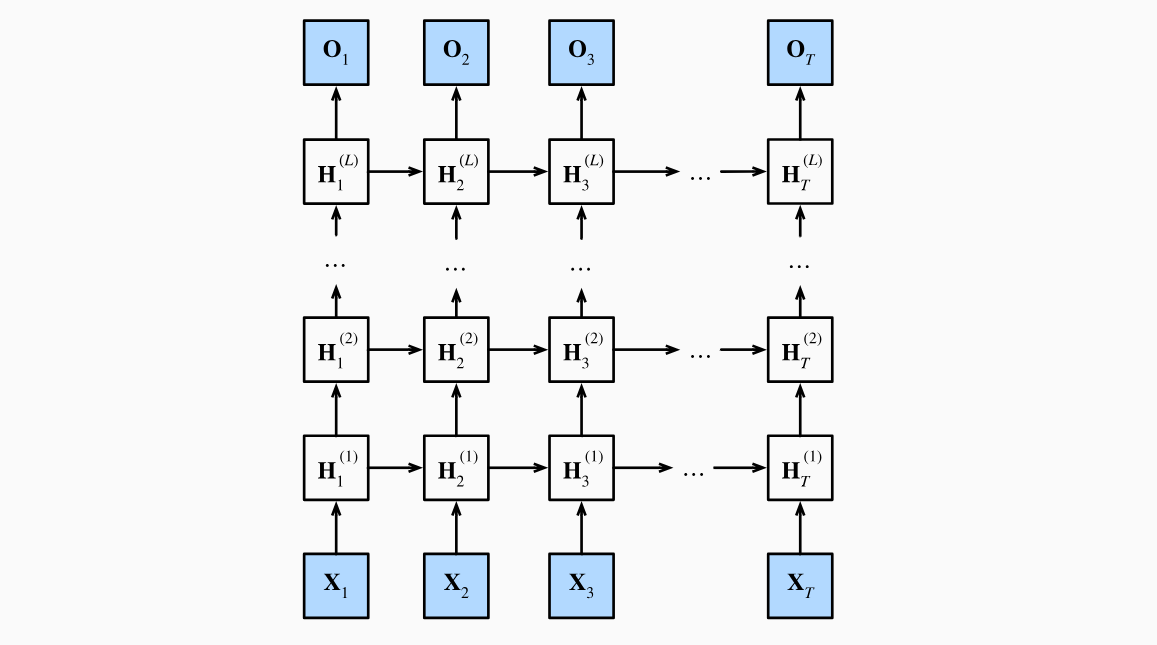
\includegraphics{images/image-0008.png}
\caption{深度循环神经网络结构}
\end{figure}

我们可以将深度架构中的函数依赖关系形式化，这个架构由 \(L\) 个隐藏层构成。后续的讨论主要集中在经典的循环神经网络模型上，但这些讨论也适用于其他序列模型。

假设在时间步 \(t\) 有一个小批量的输入数据 \(X_t \in \mathbb{R}^{n \times d}\)（样本数为 \(n\)，每个样本中的输入数为 \(d\)）。同时，将第 \(l\) 个隐藏层（\(l = 1, \ldots, L\)）的隐状态设为 \(H_t^{(l)} \in \mathbb{R}^{n \times h}\)（隐藏单元数为 \(h\)），输出层变量设为 \(O_t \in \mathbb{R}^{n \times q}\)（输出数为 \(q\)）。设置 \(H_t^{(0)} = X_t\)，第 \(l\) 个隐藏层的隐状态使用激活函数 \(\phi_l\)，则：

\[
H_t^{(l)} = \phi_l(H_t^{(l-1)}W_{xh}^{(l)} + H_{t-1}^{(l)}W_{hh}^{(l)} + b_h^{(l)})
\]

其中，权重 \(W_{xh}^{(l)} \in \mathbb{R}^{h \times h}\)、\(W_{hh}^{(l)} \in \mathbb{R}^{h \times h}\) 和偏置 \(b_h^{(l)} \in \mathbb{R}^{1 \times h}\) 都是第 \(l\) 个隐藏层的模型参数。

最后，输出层的计算仅基于第 \(L\) 个隐藏层最终的隐状态：

\[
O_t = H_t^{(L)}W_{hq} + b_q
\]

其中，权重 \(W_{hq} \in \mathbb{R}^{h \times q}\) 和偏置 \(b_q \in \mathbb{R}^{1 \times q}\) 都是输出层的模型参数。

与多层感知机一样，隐藏层数目 \(L\) 和隐藏单元数目 \(h\) 都是超参数，可以由我们调整。另外，用门控循环单元或长短期记忆网络的隐状态来代替上式中的隐状态进行计算，可以很容易地得到深度门控循环神经网络或深度长短期记忆神经网络。

\hypertarget{ux53c2ux8003ux6587ux732e-20}{%
\subsection{参考文献}\label{ux53c2ux8003ux6587ux732e-20}}

\begin{itemize}
\tightlist
\item
  Aston Zhang, Zachary C. Lipton, Mu Li, Alexander J. Smola. (2023). \href{https://zh.d2l.ai/}{《动手学深度学习》}. Cambridge University Press.
\end{itemize}

\clearpage

\hypertarget{ux53ccux5411ux5faaux73afux795eux7ecfux7f51ux7edc}{%
\section{双向循环神经网络}\label{ux53ccux5411ux5faaux73afux795eux7ecfux7f51ux7edc}}

\hypertarget{ux4e00ux9690ux9a6cux5c14ux53efux592bux6a21ux578bux4e2dux7684ux52a8ux6001ux89c4ux5212}{%
\subsection{一、隐马尔可夫模型中的动态规划}\label{ux4e00ux9690ux9a6cux5c14ux53efux592bux6a21ux578bux4e2dux7684ux52a8ux6001ux89c4ux5212}}

如果我们想用概率图模型来解决这个问题，可以设计一个隐变量模型：在任意时间步 \(t\)，假设存在某个隐变量 \(h_t\)，通过概率 \(P(x_t \mid h_t)\) 控制我们观测到的 \(x_t\)。此外，任何 \(h_t \to h_{t+1}\) 转移都由一些状态转移概率 \(P(h_{t+1} \mid h_t)\) 给出。这个概率图模型就是一个隐马尔可夫模型（hidden Markov model，HMM），如下图所示。

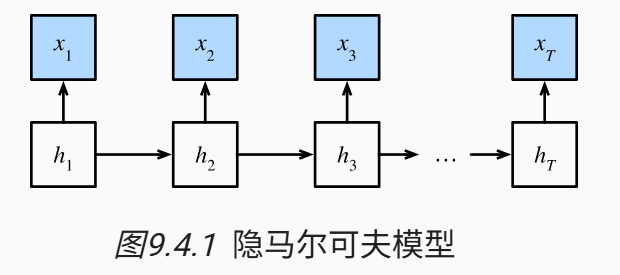
\includegraphics{images/image-0009.png}

因此，对于有 \(T\) 个观测值的序列，我们在观测状态和隐状态上具有以下联合概率分布：

\[
P(x_1, \ldots, x_T, h_1, \ldots, h_T)
= \prod_{t=1}^{T} P(h_t \mid h_{t-1})P(x_t \mid h_t), \quad P(h_1 \mid h_0) = P(h_1)
\]

现在，假设我们观测到所有的 \(x_i\)，除了 \(x_j\)，并且我们的目标是计算 \(P(x_j \mid x_{-j})\)，其中 \(x_{-j} = (x_1, \ldots, x_{j-1}, x_{j+1}, \ldots, x_T)\)。由于 \(P(x_j \mid x_{-j})\) 中没有隐变量，因此我们考虑对 \(h_1, \ldots, h_T\) 选择构成的所有可能的组合进行求和。如果任何 \(h_i\) 可以接受 \(k\) 个不同的值（有限的状态数），这意味着我们需要对 \(k^T\) 个项求和，这个任务显然难于登天。幸运的是，有个巧妙的解决方案：动态规划（dynamic programming）。

\begin{enumerate}
\def\labelenumi{\arabic{enumi}.}
\tightlist
\item
  前向递归（``对上次递推''）
\end{enumerate}

为了理解动态规划的工作方式，我们考虑对隐变量 \(h_1, \ldots, h_T\) 的依次求和。根据上面的联合分布可得：

\[
\begin{aligned}
P(x_1, \ldots, x_T)
&= \sum_{h_1,\ldots,h_T} P(x_1, \ldots, x_T, h_1, \ldots, h_T) \\
&= \sum_{h_1,\ldots,h_T} \prod_{t=1}^{T} P(h_t \mid h_{t-1})P(x_t \mid h_t) \\
&= \sum_{h_2,\ldots,h_T}\left[\sum_{h_1}P(h_1)P(x_1 \mid h_1)P(h_2 \mid h_1)\right]P(x_2 \mid h_2)\prod_{t=3}^{T}P(h_t \mid h_{t-1})P(x_t \mid h_t) \\
&= \sum_{h_3,\ldots,h_T}\left[\sum_{h_2}\pi_2(h_2)P(x_2 \mid h_2)P(h_3 \mid h_2)\right]P(x_3 \mid h_3)\prod_{t=4}^{T}P(h_t \mid h_{t-1})P(x_t \mid h_t) \\
&= \ldots \\
&= \sum_{h_T}\pi_T(h_T)P(x_T \mid h_T)
\end{aligned}
\]

其中，\(\pi_t(h_t)\) 表示所有得到 \((h_1, \ldots, h_{t-1}, h_t, x_1, \ldots, x_{t-1})\) 的路径概率之和。换句话说，它是在已观测 \(x_1, \ldots, x_{t-1}\) 后到达 \(t\) 时刻隐状态 \(h_t\) 的累计概率。因此，最后只需要对 \(h_T\) 求和即可。

通常，我们将前向递归（forward recursion）写为：

\[
\pi_{t+1}(h_{t+1}) = \sum_{h_t}\pi_t(h_t)P(x_t \mid h_t)P(h_{t+1} \mid h_t)
\]

递归被初始化为 \(\pi_1(h_1) = P(h_1)\)。符号简化后，也可以写成 \(\pi_{t+1} = f(\pi_t, x_t)\)，其中 \(f\) 是一些可学习的函数。这看起来就像我们在循环神经网络中讨论的隐变量模型中的更新方程。

\begin{enumerate}
\def\labelenumi{\arabic{enumi}.}
\setcounter{enumi}{1}
\tightlist
\item
  后向递归（``对下次递推''）
\end{enumerate}

这里我们设的 \(\rho_t(h_t)\) 是``在已经得到 \(h_t, x_t\) 条件下，最终得到 \((x_{t+1}, \ldots, x_T)\) 的概率''，是``给定状态下的预测概率''，包含了对经过的各种可能的 \(h_{t+1}, \ldots, h_T\) 路径概率的求和。

为了反向进行动态规划，可以从序列末尾逐步把未来路径的概率合并到 \(\rho\) 中：

\[
\begin{aligned}
P(x_1, \ldots, x_T)
&= \sum_{h_1,\ldots,h_T} P(x_1, \ldots, x_T, h_1, \ldots, h_T) \\
&= \sum_{h_1,\ldots,h_T}\prod_{t=1}^{T-1}P(h_t \mid h_{t-1})P(x_t \mid h_t)\cdot P(h_T \mid h_{T-1})P(x_T \mid h_T) \\
&= \sum_{h_1,\ldots,h_{T-1}}\prod_{t=1}^{T-1}P(h_t \mid h_{t-1})P(x_t \mid h_t)\cdot \left[\sum_{h_T}P(h_T \mid h_{T-1})P(x_T \mid h_T)\right] \\
&= \sum_{h_1,\ldots,h_{T-2}}\prod_{t=1}^{T-2}P(h_t \mid h_{t-1})P(x_t \mid h_t)\cdot \left[\sum_{h_{T-1}}P(h_{T-1} \mid h_{T-2})P(x_{T-1} \mid h_{T-1})\rho_{T-1}(h_{T-1})\right] \\
&= \ldots \\
&= \sum_{h_1}P(h_1)P(x_1 \mid h_1)\rho_1(h_1)
\end{aligned}
\]

因此，我们可以将后向递归（backward recursion）写为：

\[
\rho_{t-1}(h_{t-1}) = \sum_{h_t}P(h_t \mid h_{t-1})P(x_t \mid h_t)\rho_t(h_t)
\]

注：这里 \(\rho_1(h_1)\) 内部已经包含了对经过各种 \(h_2, \ldots, h_T\) 路径的求和。

为保证 \(t=T\) 时公式形式的一致性，初始化 \(\rho_T(h_T)=1\)。前向和后向递归都允许我们对 \(T\) 个隐变量在 \(O(kT)\)（线性而不是指数）时间内对 \((h_1,\ldots,h_T)\) 的所有值求和，这是使用图模型进行概率推理的巨大好处之一。它也是通用消息传递算法的一个非常特殊的例子。

\begin{enumerate}
\def\labelenumi{\arabic{enumi}.}
\setcounter{enumi}{2}
\tightlist
\item
  二者的结合
\end{enumerate}

如果我们只知道时间序列输出 \(x_1,\ldots,x_T\) 中除了 \(x_j\) 之外其他所有元素，但不知道隐状态 \(h_1,\ldots,h_T\)，这时如果逐个枚举每个 \(h_j\) 的全部可取的值（假设每个 \(h_j\) 的取值空间有 \(k\) 个值），其计算复杂度为 \(O(k^T)\)，显然行不通。

这里我们采用前向递归与后向递归结合的方法：

\[
P(x_j \mid x_{-j}) \propto \sum_{h_j}\pi_j(h_j)\rho_j(h_j)P(x_j \mid h_j)
\]

这里分母是得到除了 \(x_j\) 之外其他所有元素的概率，是和隐状态无关的常数。因为符号简化的需要，后向递归也可以写为 \(\rho_{t-1}=g(\rho_t,x_t)\)，其中 \(g\) 是一个可以学习的函数。同样，这看起来非常像一个更新方程，只是它不像我们在循环神经网络中看到的那样是前向运算，而是后向计算。事实上，知道未来数据何时可用对隐马尔可夫模型是有益的；信号处理学家将是否知道未来观测这种情况区分为内插和外推。

从计算复杂度的角度，无论是前向递归还是后向递归，对 \(T\) 个隐变量的情况对 \((h_1,\ldots,h_T)\) 的所有取值情况求和，递归计算过程的计算复杂度均为 \(O(kT)\)。上述公式相当于 \(x_j\) 以前取前向递归，以后取后向递归，计算复杂度仍然为 \(O(kT)\)。（注：这里的计算复杂度是执行计算时的，并不包括训练阶段训练概率值之类的）

\hypertarget{ux4e8cux53ccux5411ux5faaux73afux795eux7ecfux7f51ux7edc}{%
\subsection{二、双向循环神经网络}\label{ux4e8cux53ccux5411ux5faaux73afux795eux7ecfux7f51ux7edc}}

在序列学习中，我们以往假设的目标是：在给定观测的情况下（例如，在时间序列的上下文中或在语言模型的上下文中）， 对下一个输出进行建模。但实际上，对于文章挖空填空这样的任务，每个短语的``下文''传达了重要信息（如果有的话），而这些信息关乎到选择哪个词来填空， 所以无法利用这一点的序列模型将在相关任务上表现不佳。例如，如果要做好命名实体识别 （例如，识别``Green''指的是``格林先生''还是绿色）， 不同长度的上下文范围重要性是相同的。

对于任意时间步 \(t\)，给定一个小批量的输入数据 \(\mathbf{X}_t \in \mathbb{R}^{n \times d}\)（样本数 \(n\)，每个示例中的输入数 \(d\)），并且令隐藏层激活函数为 \(\phi\)。

在双向架构中，我们设该时间步的前向和反向隐状态分别为 \(\overrightarrow{\mathbf{H}}_t \in \mathbb{R}^{n \times h}\) 和 \(\overleftarrow{\mathbf{H}}_t \in \mathbb{R}^{n \times h}\)，其中 \(h\) 是隐藏单元的数目。前向和反向隐状态的更新如下：

\[
\begin{aligned}
\overrightarrow{\mathbf{H}}_t &= \phi(\mathbf{X}_t\mathbf{W}_{xh}^{(f)} + \overrightarrow{\mathbf{H}}_{t-1}\mathbf{W}_{hh}^{(f)} + \mathbf{b}_h^{(f)}), \\
\overleftarrow{\mathbf{H}}_t &= \phi(\mathbf{X}_t\mathbf{W}_{xh}^{(b)} + \overleftarrow{\mathbf{H}}_{t+1}\mathbf{W}_{hh}^{(b)} + \mathbf{b}_h^{(b)})
\end{aligned}
\]

其中，权重 \(\mathbf{W}_{xh}^{(f)} \in \mathbb{R}^{d \times h}\)、\(\mathbf{W}_{hh}^{(f)} \in \mathbb{R}^{h \times h}\)、\(\mathbf{W}_{xh}^{(b)} \in \mathbb{R}^{d \times h}\)、\(\mathbf{W}_{hh}^{(b)} \in \mathbb{R}^{h \times h}\) 和偏置 \(\mathbf{b}_h^{(f)} \in \mathbb{R}^{1 \times h}\)、\(\mathbf{b}_h^{(b)} \in \mathbb{R}^{1 \times h}\) 都是模型参数。

接下来，将前向隐状态 \(\overrightarrow{\mathbf{H}}_t\) 和反向隐状态 \(\overleftarrow{\mathbf{H}}_t\) 连接起来，获得需要送入输出层的隐状态 \(\mathbf{H}_t \in \mathbb{R}^{n \times 2h}\)。在具有多个隐藏层的深度双向循环神经网络中，该信息作为输入传递到下一个双向层。最后，输出层计算得到的输出为 \(\mathbf{O}_t \in \mathbb{R}^{n \times q}\)（\(q\) 是输出单元的数目）：

\[
\mathbf{O}_t = \mathbf{H}_t\mathbf{W}_{hq} + \mathbf{b}_q
\]

这里，权重矩阵 \(\mathbf{W}_{hq} \in \mathbb{R}^{2h \times q}\) 和偏置 \(\mathbf{b}_q \in \mathbb{R}^{1 \times q}\) 是输出层的模型参数。事实上，这两个方向可以拥有不同数量的隐藏单元。

双向循环神经网络的一个关键特性是：使用来自序列两端的信息来估计输出。也就是说，我们使用来自过去和未来的观测信息来预测当前的观测。但是在对下一个词元进行预测的情况中，这样的模型并不是我们所需的。因为在预测下一个词元时，我们终究无法知道下一个词元的下文是什么，所以将不会得到很好的精度。具体地说，在训练期间，我们能够利用过去和未来的数据来估计现在空缺的词；而在测试期间，我们只有过去的数据，因此精度将会很差。下面的实验将说明这一点。

另一个严重问题是，双向循环神经网络的计算速度非常慢。其主要原因是网络的前向传播需要在双向层中进行前向和后向递归，并且网络的反向传播还依赖于前向传播的结果。因此，梯度求解将有一个非常长的链。

双向层的使用在实践中非常少，并且仅仅应用于部分场合。例如，填充缺失的单词、词元注释（例如，用于命名实体识别），以及作为序列处理流水线中的一个步骤对序列进行编码（例如，用于机器翻译）。在相关后续章节中，将介绍如何使用双向循环神经网络编码文本序列。

\hypertarget{ux53c2ux8003ux6587ux732e-21}{%
\subsection{参考文献}\label{ux53c2ux8003ux6587ux732e-21}}

\begin{itemize}
\tightlist
\item
  Aston Zhang, Zachary C. Lipton, Mu Li, Alexander J. Smola. (2023). \href{https://zh.d2l.ai/}{《动手学深度学习》}. Cambridge University Press.
\item
  Schuster, M., \& Paliwal, K. K. (1997). \href{https://doi.org/10.1109/78.650093}{Bidirectional recurrent neural networks}. IEEE Transactions on Signal Processing.
\end{itemize}

\clearpage

\hypertarget{ux5e8fux5217ux5230ux5e8fux5217seq2sequx5b66ux4e60}{%
\section{序列到序列（Seq2Seq）学习}\label{ux5e8fux5217ux5230ux5e8fux5217seq2sequx5b66ux4e60}}

从技术上讲，编码器将长度可变的输入序列转换成形状固定的上下文变量 \(\mathbf{c}\)，并且将输入序列的信息在该上下文变量中进行编码。可以使用循环神经网络来设计编码器。

考虑由一个序列组成的样本（批量大小是 1）。假设输入序列是 \(x_1,\ldots,x_T\)，其中 \(x_t\) 是输入文本序列中的第 \(t\) 个词元。在时间步 \(t\)，循环神经网络将词元 \(x_t\) 的输入特征向量 \(\mathbf{x}_t\) 和 \(\mathbf{h}_{t-1}\)（即上一时间步的隐状态）转换为 \(\mathbf{h}_t\)（即当前步的隐状态）。使用一个函数 \(f\) 来描述循环神经网络的循环层所做的变换：

\[
\mathbf{h}_t = f(\mathbf{x}_t,\mathbf{h}_{t-1})
\]

总之，编码器通过选定的函数 \(q\)，将所有时间步的隐状态转换为上下文变量：

\[
\mathbf{c} = q(\mathbf{h}_1,\ldots,\mathbf{h}_T)
\]

正如上文提到的，编码器输出的上下文变量 \(\mathbf{c}\) 对整个输入序列 \(x_1,\ldots,x_T\) 进行编码。来自训练数据集的输出序列 \(y_1,y_2,\ldots,y_{T'}\)，对于每个时间步 \(t'\)（与输入序列或编码器的时间步 \(t\) 不同），解码器输出 \(y_{t'}\) 的概率取决于先前的输出子序列 \(y_1,\ldots,y_{t'-1}\) 和上下文变量 \(\mathbf{c}\)，即 \(P(y_{t'} \mid y_1,\ldots,y_{t'-1},\mathbf{c})\)。

为了在序列上模型化这种条件概率，我们可以使用另一个循环神经网络作为解码器。在输出序列上的任意时间步 \(t'\)，循环神经网络将来自上一时间步的输出 \(y_{t'-1}\) 和上下文变量 \(\mathbf{c}\) 作为其输入，然后在当前时间步将它们和上一隐状态 \(\mathbf{s}_{t'-1}\) 转换为隐状态 \(\mathbf{s}_{t'}\)。因此，可以使用函数 \(g\) 表示解码器的隐藏层的变换：

\[
\mathbf{s}_{t'} = g(y_{t'-1},\mathbf{c},\mathbf{s}_{t'-1})
\]

在获得解码器的隐状态之后，我们可以使用输出层和 softmax 操作来计算在时间步 \(t'\) 时输出 \(y_{t'}\) 的条件概率分布 \(P(y_{t'} \mid y_1,\ldots,y_{t'-1},\mathbf{c})\)。

在每个时间步，解码器预测了输出词元的概率分布。类似于语言模型，可以使用softmax来获得分布，并通过计算交叉熵损失函数来进行优化。另外，为了让不同长度的序列可以以相同形状的小批量加载。 特定的填充词元被添加到序列的末尾， 我们应该将填充词元的预测排除在损失函数的计算之外。用sequence\_mask函数可通过零值化屏蔽不相关的项， 以便后面任何不相关预测的计算都是与零的乘积，结果都等于零（交叉熵损失-sigma(pi*logqi),pi=0）。

\hypertarget{ux53c2ux8003ux6587ux732e-22}{%
\subsection{参考文献}\label{ux53c2ux8003ux6587ux732e-22}}

\begin{itemize}
\tightlist
\item
  Aston Zhang, Zachary C. Lipton, Mu Li, Alexander J. Smola. (2023). \href{https://zh.d2l.ai/}{《动手学深度学习》}. Cambridge University Press.
\end{itemize}

\clearpage
